%!TEX root = 00_main.tex

\section{Introduction}

% \commentA{would be nice to show the process figure as a teaser above abstract as in the disney paper}
% Looks like the template doesn't allow us to do this easily unfortunately :(

Machine learning methods that leverage large amounts of training data currently perform best for many problems in computer vision, such as object detection, scene recognition, or gaze estimation~\cite{zhou2014learning,girshick2014rich,zhang15_cvpr}.
However, capturing or collecting large-scale training data can be time-consuming
%, especially for new areas of research without pre-existing datasets.
and supervised learning methods additionally require accurate ground truth annotation for each image.
This annotation process can be expensive and tedious, and there is no guarantee that human-provided labels will be correct.
Ground truth annotation is particularly challenging and error-prone for learning tasks that require highly fine-grained and accurate labels, such as tracking facial landmarks for facial expression analysis and gaze estimation~\todo{REF}, or body joints for pose estimation and activity recognition~\todo{REF}.

\begin{figure}
    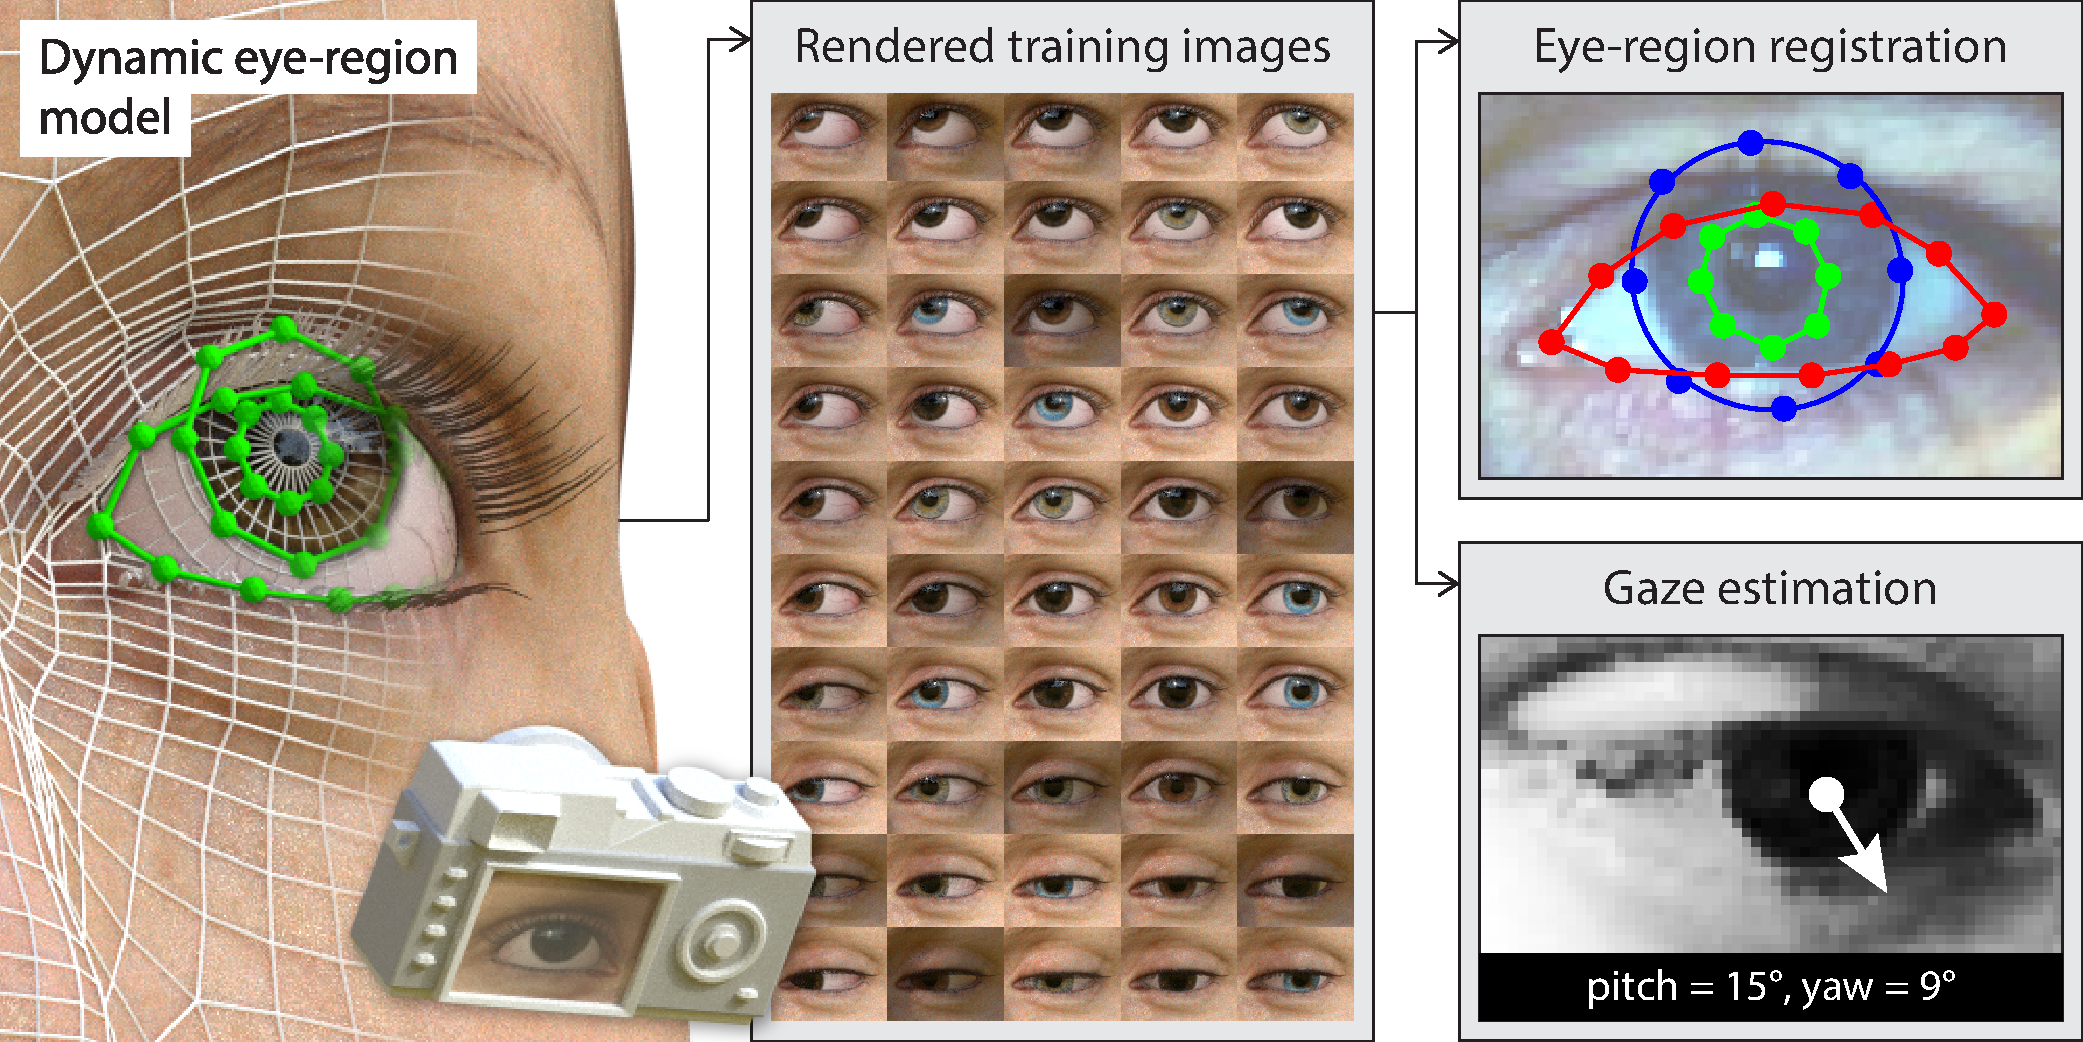
\includegraphics[width=\columnwidth]{teaser}
    \caption{At the core of our method is a dynamic eye-region model that allows us to render large numbers of photorealistic eye images as training data for eye region registration and gaze estimation.}
    \label{fig:teaser}
\end{figure}

% \commentE{The further back I look, rendering RGB training images does go back into the past for pose-estimation at least, though none of it was ``photorealistic''}
To address these problems, researchers have employed \emph{learning-by-synthesis} techniques to generate large amounts training data with computer graphics.
The advantages of this approach are that both data collection and annotation require little human labour and image synthesis can be geared to specific application scenarios.
Perhaps the best known example is by \citet{shotton2013real}, who synthesized a large and varied depth-image dataset for training a real-time pose-estimator.

The eyes and their movements are important for a range of applications including gaze-based human-computer interaction~\cite{majaranta14_apc}, visual behaviour monitoring~\cite{bulling13_chi,bulling11_pami}, and -- more recently -- computer vision tasks, such as object recognition and detection~\cite{yun2013studying,papadopoulos2014training,karthikeyan2013and}.
\commentA{we can also remove these last references if we have to save space}
Recent work by \citet{sugano2014learning} demonstrated the benefits of learning-by-synthesis for appearance-based gaze estimation, but employed only fundamental computer graphics techniques for synthesising low-resolution meshes that did not account for lighting variation.
% \commentY{Mentioning "shape changes" is misleading. UT dataset us just {\em discrete} in terms of gaze directions and eyelid movements, and it has larger variety of facial shape variations (50 persons), and eyelid deformation is anatomically correct. In my impression, shape variation is still a weak point of this work.}
The eye-region is particularly difficult to model accurately given the dynamic shape changes it undergoes with facial motion and eyeball rotation, and the complex material structure of the eyeball itself.
It is for this reason that previous work on rendering photorealistic images of the eye and eye-region is relatively sparse~\cite{ActiBlizEyes,berard2014highquality}.

controllability
illumination

\commentY{What does this "sparsity" mean? And again, I think having 10 different models is a little to weak to say that it can handle "significant variation in facial shape and texture across different people" in the context of face/eye research.}

\todo{final sentence on limitations of existing models in this area}

\commentA{we also need to motivate why high quality renderings are needed, i.e. why it's worthwhile to put so much effort into the model. And later we can hopefully also show that it pays off to do so...}

% Andreas: we need some transition to eyeballs here, e.g. eyeball rendering is particularly challenging and interesting because of the many muscles involved, the large number of appearance details around and in the eye etc.
% essentially motivate that this hasn't been done before and is a very interesting area of research

%Synthesising training data is not novel in itself -- previous work has ... Our novel approach 

We present a novel method for photorealistic rendering of full face and eye images at a large scale using a collection of dynamic eye-region models.
In contrast to previous works, we provide a comprehensive and detailed description of the model preparation process and rendering pipeline.
We then present and evaluate two separate systems trained on \dataset: a novel eye-region specific deformable model and an appearance-based gaze estimator.
These systems are case studies that show how we leverage the degrees of control made available by rendering our training data to easily and quickly generate high quality training datasets.

The specific contributions of this work are threefold. First, \todo{...}
We present our dynamic eye-region model that uses multiple parts and blend shapes to model the continuous degrees of shape change and deformation exhibited by the eye.
We then present a novel application of learning-by-synthesis: eye-region registration.